\pgfplotstablegetelem{\thepart}{[index]\columnIndex}\of{\cronograma}
\part{\pgfplotsretval}
\label{part:\thepart}
\frame{\partpage}


%\section{Conceitos}
%

\begin{frame}[t]{Apresentação e boas-vindas}
	\fontsize{14pt}{15.2}\selectfont{
		Olá?  \\
		
	 
	}\par
	\vspace{1em}
	
	
\end{frame}




\begin{frame}[t]{Desafio}
	\fontsize{10pt}{10}\selectfont{
		* A = Passo a frente, * B = Vire para a direita, * C = Vire para a esquerda 
	}
	\centering
	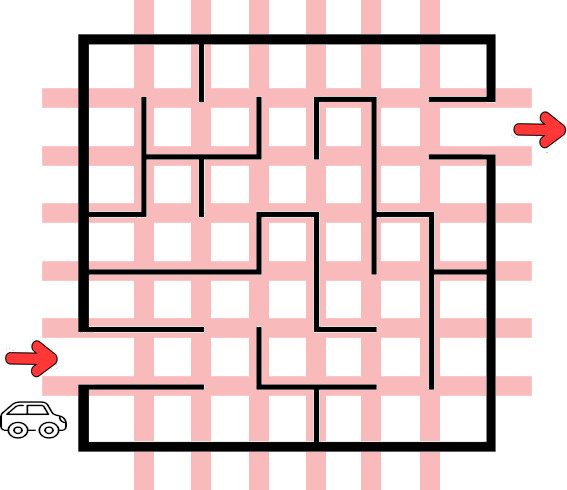
\includegraphics[scale=1.6]{imagens/fig-labirinto.jpg}
	
\end{frame}


\begin{frame}{Desafio}
	
	
	\begin{multicols}{2}
		\fontsize{10pt}{12}\selectfont{
			
			A - Passo a frente\\
			A - Passo a frente\\
			A - Passo a frente\\
			C - Vire para a esquerda\\
			A - Passo a frente\\
			B - Vire para a direita\\
			A - Passo a frente\\
			C - Vire para a esquerda\\
			A - Passo a frente\\
			A - Passo a frente\\
			
		}\par
		\columnbreak
		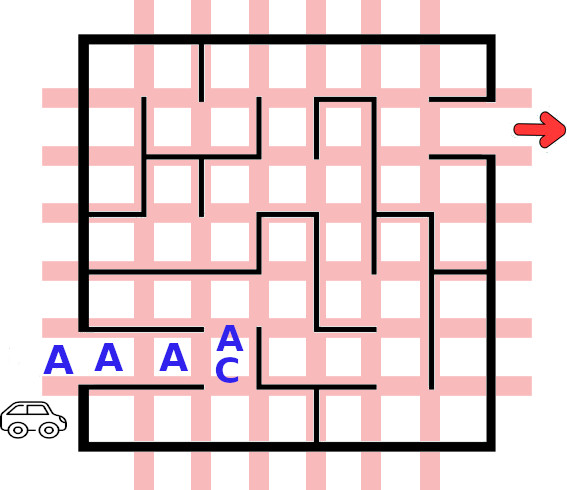
\includegraphics[scale=1.2]{imagens/fig-labirinto2.jpg}
		
	\end{multicols}
	
	
\end{frame}




\begin{frame}[t]{Lógica de Programação com Django}
	\fontsize{14pt}{15.2}\selectfont{
		A lógica de programação é a forma como são conduzidas as ações realizadas por algoritmos.  \\
		
		
	}\par
	\vspace{1em}
	
	\fontsize{12pt}{15}\selectfont{
		\begin{itemize}%[<+->]  
			\item Toda programação apresenta um encadeamento lógico para que os códigos descritos possam executar os comandos atribuídos. 
			
			\item Nesse sentido, quem programa é responsável por compreender essa lógica e traduzi-la de forma eficiente para a máquina.
			
			
			
		\end{itemize}
	}\par
	\vspace{1em}
	
\end{frame}




\begin{frame}[t]{Exercícios}
	
	
	\fontsize{10pt}{15}\selectfont{
		\begin{itemize}%[<+->]  
			
			\item \glsfirst{exercicio_001}: \glsdesc{exercicio_001}
			
			\item \glsfirst{exercicio_002}: \glsdesc{exercicio_002}
			
			\item \glsfirst{exercicio_003}: \glsdesc{exercicio_003}
			
			\item \glsfirst{exercicio_004}: \glsdesc{exercicio_004}
			
		\end{itemize}
	}\par
	\vspace{1em}
	
\end{frame}


